\documentclass[11pt,a4paper]{article}
\usepackage[T1]{fontenc}
\usepackage[utf8]{inputenc}
\usepackage{lmodern}
\usepackage{amsmath,amssymb,amsthm,mathtools,mathrsfs}
\usepackage{graphicx,float,xcolor,multicol}
\usepackage[shortlabels]{enumitem}
\usepackage[margin=27mm]{geometry}
\usepackage{microtype,needspace,placeins}
\usepackage{tikz,tikz-cd}
\usetikzlibrary{arrows.meta,calc,positioning,patterns,decorations.pathreplacing}
\usepackage[colorlinks=true,linkcolor=teal,urlcolor=teal,citecolor=teal]{hyperref}
\setlength{\parindent}{0pt}
\setlength{\parskip}{.6em}
\setcounter{secnumdepth}{0}
\allowdisplaybreaks
\raggedbottom
\providecommand{\cross}{\times}
\DeclareUnicodeCharacter{2020}{\ensuremath{\dagger}}
\DeclareMathOperator{\supp}{supp}
\DeclareMathOperator*{\esssup}{ess\,sup}
\providecommand{\chapter}{\section}
\newenvironment{tool}[2]{\subsection*{Tool #1 --- #2}}{}
\newcommand{\ToolRef}[1]{Tool #1}
\newcommand{\FigureTag}[2]{\textit{Figure #1}}
\newcommand{\Result}[1]{\subsection*{#1}}
\newcommand{\Application}[1]{\subsubsection*{Application\if\relax\detokenize{#1}\relax\else\space--- #1\fi}}
\newcommand{\ProofHeading}{\par\textit{Proof.}\space}
\newcommand{\ProofOf}[1]{\par\textit{Proof of #1.}\space}
\newcommand{\RemarkHeading}{\par\textbf{Remark.}\space}
\newcommand{\NoteHeading}{\par\textbf{Note.}\space}
\newcommand{\ExerciseHeading}{\par\textbf{Exercise.}\space}

% Rendering support only; mathematical text is in each independent post.
\usepackage{booktabs,array,longtable}
\definecolor{HandoutBlue}{HTML}{2F6690}
\definecolor{HandoutNavy}{HTML}{17365D}
\newtheorem{theorem}{Theorem}
\newtheorem{lemma}[theorem]{Lemma}
\newtheorem{proposition}[theorem]{Proposition}
\newtheorem{corollary}[theorem]{Corollary}
\newtheorem{conjecture}[theorem]{Conjecture}
\newtheorem{definition}{Definition}
\newtheorem{example}{Example}
\newtheorem{namedtoolcounter}{Tool}
\newenvironment{namedtool}[1]{\begin{namedtoolcounter}[#1]}{\end{namedtoolcounter}}
\newtheorem*{claim}{Claim}
\newtheorem*{remark}{Remark}
\newtheorem*{exercise}{Exercise}
\newtheorem*{question}{Question}
\newtheorem*{observation}{Observation}
\newcommand{\SourceChapter}[2]{\section*{#2}}
\newcommand{\Lecture}[2]{\section*{Lecture #1: #2}}
\newcommand{\unclear}[1]{\textit{[unclear: #1]}}
\newcommand{\sourcegap}{\textit{[unfinished in the source]}}
\DeclareMathOperator{\dist}{dist}
\DeclareMathOperator{\id}{id}
\DeclareMathOperator{\Hol}{Hol}
\DeclareMathOperator{\Per}{Per}
\DeclareMathOperator{\Fix}{Fix}
\DeclareMathOperator{\diam}{diam}
\DeclareMathOperator{\Var}{Var}
\DeclareMathOperator{\Leb}{Leb}
\DeclareMathOperator{\Hom}{Hom}
\DeclareMathOperator{\End}{End}
\DeclareMathOperator{\Ann}{Ann}
\DeclareMathOperator{\Spec}{Spec}
\DeclareMathOperator{\Max}{Max}
\DeclareMathOperator{\Ob}{Ob}
\DeclareMathOperator{\Tor}{Tor}
\DeclareMathOperator{\Ass}{Ass}
\DeclareMathOperator{\Mor}{Mor}
\DeclareMathOperator{\Fun}{Fun}
\DeclareMathOperator{\Nat}{Nat}
\DeclareMathOperator{\Cone}{Cone}
\DeclareMathOperator{\MCG}{MCG}
\DeclareMathOperator{\Aut}{Aut}
\DeclareMathOperator{\Deck}{Deck}
\DeclareMathOperator{\SL}{SL}
\DeclareMathOperator{\PSL}{PSL}
\DeclareMathOperator{\Area}{Area}
\DeclareMathOperator{\im}{im}
\DeclareMathOperator{\PSh}{PSh}
\newcommand{\CRing}{\mathsf{CRings}}
\newcommand{\AMod}{A\text{-}\mathsf{Mod}}
\newcommand{\Ab}{\mathsf{Ab}}
\newcommand{\Z}{\mathbb Z}
\newcommand{\Q}{\mathbb Q}
\newcommand{\R}{\mathbb R}
\newcommand{\C}{\mathbb C}
\newcommand{\N}{\mathbb N}
\newcommand{\kk}{\mathbb k}
\renewcommand{\aa}{\mathfrak a}
\newcommand{\bb}{\mathfrak b}
\newcommand{\pp}{\mathfrak p}
\newcommand{\qq}{\mathfrak q}
\newcommand{\mm}{\mathfrak m}
\newcommand{\nn}{\mathfrak n}
\newcommand{\rad}{\mathrm r}
\newcommand{\cat}[1]{\mathsf{#1}}
\setcounter{secnumdepth}{0}
\allowdisplaybreaks

\graphicspath{{figures/complex-dynamics-notes/}}
\begin{document}
\section*{Attracting and Repelling Fixed Points}
% BLOG-CONTENT-BEGIN
In this exposition we are interested only in the local behaviour of a holomorphic map $f\colon S\to S$, where $S$ is a Riemann surface. For this, it would ``suffice'' to study the local behaviour at fixed points of $f$. Recall that $S$ decomposes into components of basins with fractal-like boundaries (elements of the Julia set). Our goal is to describe the dynamics of $f$ locally in certain such basins. The underlying phenomenon governing these dynamics is the distribution of the critical points of $f$, especially for rational maps on $\widehat{\mathbb C}$. We shall explain this phenomenon.

Understanding the dynamics near fixed points amounts to finding a change of coordinates in which the orbits of $f$ are easy to describe, as expected. A general technique is to construct a local biholomorphism $\phi$ such that the following diagram commutes.
\begin{figure}[H]\centering
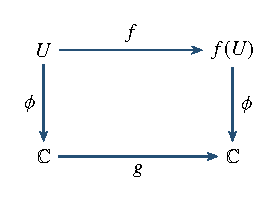
\includegraphics[width=.32\textwidth]{cd2-fig-01.pdf}
\FigureTag{CD2.1}{fig:cd2-01}
\end{figure}
% Source page 2
That is, $\phi\circ f\circ\phi^{-1}=g$ locally around $0$, where $g$ is preferably a polynomial. One begins by finding maps $\{\phi_k\}_k$ such that $\phi_k\circ f=g\circ\phi_{k+1}$, then proves that $\phi_k\to\phi$ uniformly. Consequently,
\[
\lim_{k\to\infty}(\phi_k\circ f)=\lim_{k\to\infty}(g\circ\phi_{k+1}),
\quad\phi\circ f=g\circ\phi,
\quad\phi\circ f\circ\phi^{-1}=g.
\]
\setcounter{definition}{6}\begin{definition}
A fixed point is \emph{superattracting} if its multiplier $\lambda$ is $0$, geometrically attracting if $0<|\lambda|<1$, and repelling if $1<|\lambda|$.
\end{definition}
We deal with all fixed points except those for which $\lambda\in S^1$. First let us understand the dynamics locally, and then describe the phenomenon governing it.
\subsection{Geometrically attracting and repelling points}
% Source page 3
\Needspace{18\baselineskip}
\setcounter{theorem}{10}\begin{theorem}[Koenigs linearisation]\label{cd2:koenigs}
If the multiplier satisfies $|\lambda|\notin\{0,1\}$, there is a map $\phi$, unique up to multiplication by a nonzero constant, such that the following diagram commutes.
\begin{figure}[H]\centering
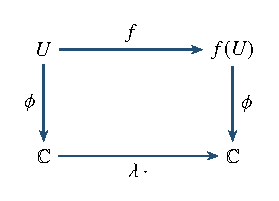
\includegraphics[width=.32\textwidth]{cd2-fig-02.pdf}
\FigureTag{CD2.2}{fig:cd2-02}
\end{figure}
\end{theorem}
\begin{proof}
\emph{Case 1: $|\lambda|<1$.} Identify $f$ with its local coordinate expression $\widehat f$. Let $0$ be the fixed point. We have $f(z)=\lambda z+O(z^2)$ in $\mathbb D_{r_0}$ for some $r_0<1$, and
\[
|f(z)|\le|\lambda z|+C|z|^2\le(|\lambda|+C|z|)|z|\qquad(|z|<r_0).
\]
Since $|\lambda|<1$, choosing $|z|$ small enough keeps $|\lambda|+C|z|$ within $\mathbb D$. More precisely, choose $0<r\le r_0$ such that $|\lambda|+Cr<1$, and put $c=|\lambda|+Cr$. Then $|f(z)|\le c|z|$ for every $z\in\mathbb D_r$, so $f(z)\in\mathbb D_r$ and
$|f^{\circ n}(z)|\le c^n|z|<c^nr\to0$ as $n\to\infty$.
% Source page 4
This is precisely the push/pull we were discussing. There is $r<1$ such that $|f(z)|<c|z|$ on $\mathbb D_r$, with $c<1$. Let $\{z_n\}_n$ be the orbit of $z_0\in\mathbb D_r$. All these orbits converge to the origin, since $|z_n|\le rc^n$, and $|z_{n+1}-\lambda z_n|\le C|z_n|^2\le Cr^2c^{2n}$. Set $w_n=z_n/\lambda^n$. Then
\begin{align*}
|w_{n+1}-w_n|
&=\left|\frac{z_{n+1}}{\lambda^{n+1}}-\frac{z_n}{\lambda^n}\right|
=\frac{|z_{n+1}-\lambda z_n|}{|\lambda|^{n+1}}\\
&\le\frac{Cr^2c^{2n}}{|\lambda|^{n+1}}
=\frac{Cr^2}{|\lambda|}\left(\frac{c^2}{|\lambda|}\right)^n.
\end{align*}
Choose $c$ with $c^2<|\lambda|<c$. The sequence $\{w_n\}_n$ is Cauchy, and its geometric bound is independent of $z_0$. The map $\phi_n(z_0)=f^{\circ n}(z_0)/\lambda^n$ is holomorphic on $\mathbb D_r$, with $\phi_n(f(z_0))=\lambda\phi_{n+1}(z_0)$. Taking $\phi=\lim_{n\to\infty}\phi_n$ gives $\phi\circ f=\lambda\phi$. Also, $\phi_n'(0)=1$, so $\phi'(0)=1$, and $\phi$ is a local conformal isomorphism around $0$.

\emph{Case 2: $|\lambda|>1$.} Since $f'(0)\ne0$, $f$ is locally invertible. Its local inverse has multiplier $0<|1/\lambda|<1$ at $0$.
% Source page 5
For uniqueness, if $\phi,\psi$ are two such Koenigs maps, then $\psi\circ\phi^{-1}$ commutes with $z\mapsto\lambda z$. If $\psi\circ\phi^{-1}(w)=\sum_{n\ge1}b_nw^n$, then $\lambda b_n=b_n\lambda^n$. Thus $b_k=0$ for every $k\ge2$, and $\psi=b_1\phi$.
\end{proof}
\subsection{Superattracting fixed points}
If $f'(0)=0$, then locally $f(z)=a_nz^n+a_{n+1}z^{n+1}+\cdots$. Thus $f$ has a zero of order $n$ at $0$, and in a suitable domain $f(z)=h(z)^nz^n$. Close to the origin in this domain, $f$ acts almost like the polynomial $a_nz^n$. The following theorem makes a much sharper claim.
\setcounter{theorem}{11}\begin{theorem}[B\"ottcher]\label{cd2:bottcher}
If $0$ is a superattracting fixed point of $f$, with a zero of order $n$ at $0$, there is a map $\phi$, unique up to multiplication by an $(n-1)$st root of unity, such that the following diagram commutes.
\begin{figure}[H]\centering
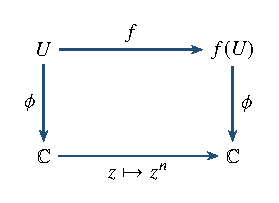
\includegraphics[width=.32\textwidth]{cd2-fig-03.pdf}
\FigureTag{CD2.3}{fig:cd2-03}
\end{figure}
\end{theorem}
% Source page 6
% Source page 8
Now that we understand the local dynamics near geometrically attracting, repelling, and superattracting points, to what extent can we extend this knowledge? In other words, on how large a domain is the nature of $f$ near these fixed points as we asserted? Let us globalise this local behaviour as far as nature allows, primarily for rational maps on $\widehat{\mathbb C}$.
\subsection{Global linearisation}
Koenigs' function $\phi$ extends holomorphically to the basin of attraction $\mathcal A$ of the fixed point $\widehat p$.
\begin{figure}[H]\centering
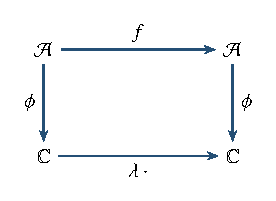
\includegraphics[width=.32\textwidth]{cd2-fig-04.pdf}
\FigureTag{CD2.4}{fig:cd2-04}
\end{figure}
\begin{proof}
The formula $\lim_{n\to\infty}f^{\circ n}(z)/\lambda^n$ is valid on $\mathcal A$, since it converges uniformly on compact sets. For every $z\in\mathcal A$, there is a neighbourhood $\overline U\subseteq\mathcal A$ on which $f^{\circ n}$ converges uniformly to $\widehat p$. Thus there is $N$ such that $f^{\circ n}(z)\in U$, the domain of $\phi$, for every $n\ge N$ and $z\in\overline U$. Then
% Source page 9
\[
\frac{\phi(f^{\circ N}(z))}{\lambda^N}
=\lim_{n\to\infty}\frac{f^{\circ n}(z)}{\lambda^n}.
\]
Indeed, $\phi$ extends to $\mathcal A$.
\end{proof}
\begin{remark}
Such an extension is not possible for B\"ottcher coordinates: to make the diagram commute one must deal with $p\mapsto\sqrt[n^k]{\phi(f^{\circ k}(p))}$, but the root is not well-defined. One can, however, extend $|\phi|$, since roots in $\mathbb R_+$ are well-defined.
\end{remark}
% Source page 10
\subsection{The phenomenon of critical points: analytic aspects}
Critical points govern rational dynamics in three significant ways:
\begin{enumerate}
\setcounter{enumi}{0}\item Critical points form the boundary beyond which Koenigs and B\"ottcher coordinates cannot be extended biholomorphically (analytic).
\setcounter{enumi}{1}\item Critical points determine the number of attracting periodic points or orbits (analytic).
\setcounter{enumi}{2}\item They determine the topological shape of the Julia set (topological; we shall see this in another exposition).
\end{enumerate}
The analysis of a rational map is essentially determined by its roots and poles, whereas in dynamics its critical points become essential. We address these phenomena one by one. Unless otherwise stated, $f$ is a rational map with $\deg(f)\ge2$, and the surface is $\widehat{\mathbb C}$.
\subsubsection{Biholomorphic extension}
\setcounter{definition}{7}\begin{definition}
Given an attracting fixed point $\widehat p$ of a map $f\colon S\to S$, let $\mathcal A_0$ denote the connected component of its basin of attraction that contains $\widehat p$.
\end{definition}
\setcounter{theorem}{12}\begin{theorem}\label{cd2:maximal}
There is a maximal $r$ such that $\psi\colon\mathbb D_r\to\mathcal A_0$ is a holomorphic inverse of the Koenigs coordinate $\phi$. The closed disc $\overline{\mathbb D_r}$ and $\psi(\overline{\mathbb D_r})$ are homeomorphic, and $\psi(\partial\mathbb D_r)$ contains a critical point of $f$.
\end{theorem}
% Source page 11
Thus critical points form the obstruction that stops, or contains, biholomorphic extension within a domain in $\mathcal A$.
% Source page 13
\begin{remark}
We defer the homeomorphism part to the next exposition, where we explore topological properties, including continuous extension to $\partial\mathbb D_r$ of the inverses of B\"ottcher and Koenigs coordinates, and much more.
\end{remark}
\subsubsection{The number of attracting periodic points}
% Source page 15
\setcounter{theorem}{14}\begin{theorem}\label{cd2:finite-attractors}
There are finitely many attracting periodic orbits.
\end{theorem}
\begin{proof}
For fixed points this follows because all immediate basins contain critical points, and a rational map has finitely many critical points. Given an attracting orbit $z_0\mapsto z_1\mapsto\cdots\mapsto z_0$ in $n$ steps, consider $f^{\circ n}$.
\end{proof}
\begin{proof}[Alternate proof]
Let $\widehat p\in O$ be an attracting fixed point, where $O$ is its immediate basin. If $O$ has no critical value of $f$, then there is a neighbourhood $U$ of $\widehat p$ and, for every $k\ge1$, a map $g_k\colon U\to\widehat{\mathbb C}$ inverse to $f^{\circ k}$. The family $\{g_k\}_k$ is normal, but $g_k'(\widehat p)$ is unbounded, since it is $\lambda^k$ with $\lambda>1$.
\end{proof}
Critical points therefore keep count of the number of attracting periodic orbits.
\setcounter{definition}{8}\begin{definition}
For $f\colon S\to S'$, a \emph{critical value} is the image under $f$ of a critical point.
\end{definition}
\setcounter{definition}{9}\begin{definition}
If there is a curve $\gamma\colon[0,1)\to S$ that eventually leaves compact sets, but $\lim_{t\to1}f(\gamma(t))=v$, then $v$ is an \emph{asymptotic value}.
\end{definition}
% Source page 16
% BLOG-CONTENT-END
\end{document}
